\chapter{Elgendiho referenční algoritmus}
\label{chap:elgendi_neurokit}

Tato kapitola popisuje, jak lze ve fotopletysmografickém (\acs{PPG}) signálu nalézt systolické vrcholy s využitím upraveného Elgendiho algoritmu, který je implementován v~knihovně NeuroKit2.
V~kapitole \ref{chap:PPG_teorie} byly již podrobně shrnuty principy \acs{PPG}, proto se zde zaměříme na vlastní detekci vrcholů a její realizaci.

\section{Obecná struktura algoritmu}
Algoritmus je možné rozdělit na dvě základní etapy: \emph{předzpracování signálu} (pásmová filtrace) a \emph{detekci systolických vrcholů} (umocnění, nastavení prahu a označení maxim).
Schéma je na obrázku \ref{fig:alg-scheme}.
Vstupem je surový fotopletysmografický záznam, zatímco výstupem jsou konkrétní časové pozice nalezených systolických vrcholů.

\begin{figure}[htbp]
	\centering
	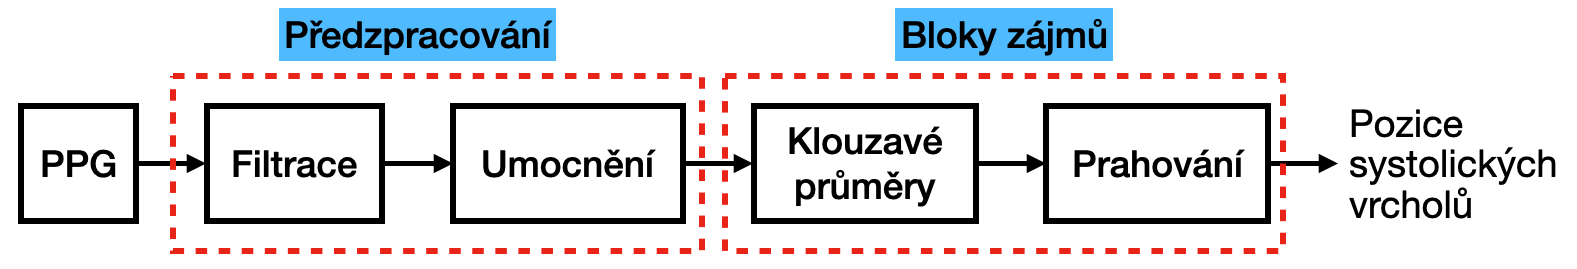
\includegraphics[width=0.8\textwidth]{./obrazky/ElgendiBlokSchema.png}
	\caption[Struktura Elgendiho algoritmu]{Zjednodušené schéma Elgendiho algoritmu.}
	\label{fig:alg-scheme}
\end{figure}

\section{Předzpracování signálu}
Před samotnou detekcí je potřeba potlačit šum a odstranit pomalé změny amplitudy.
Často se používá druhý řád Butterworthova filtru se zpracováním v~přímém i reverzním směru (tzv.~zero-phase filtering).
Frekvenční charakteristika takového filtru může být zaměřena na pásmo zhruba 0,5--8~Hz, což postačí pro typické PPG kmitočty.
Na obrázku~\ref{fig:filter-example} je ukázka amplitudové charakteristiky a zfiltrovaného úseku signálu.

\begin{figure}[htbp]
	\centering
	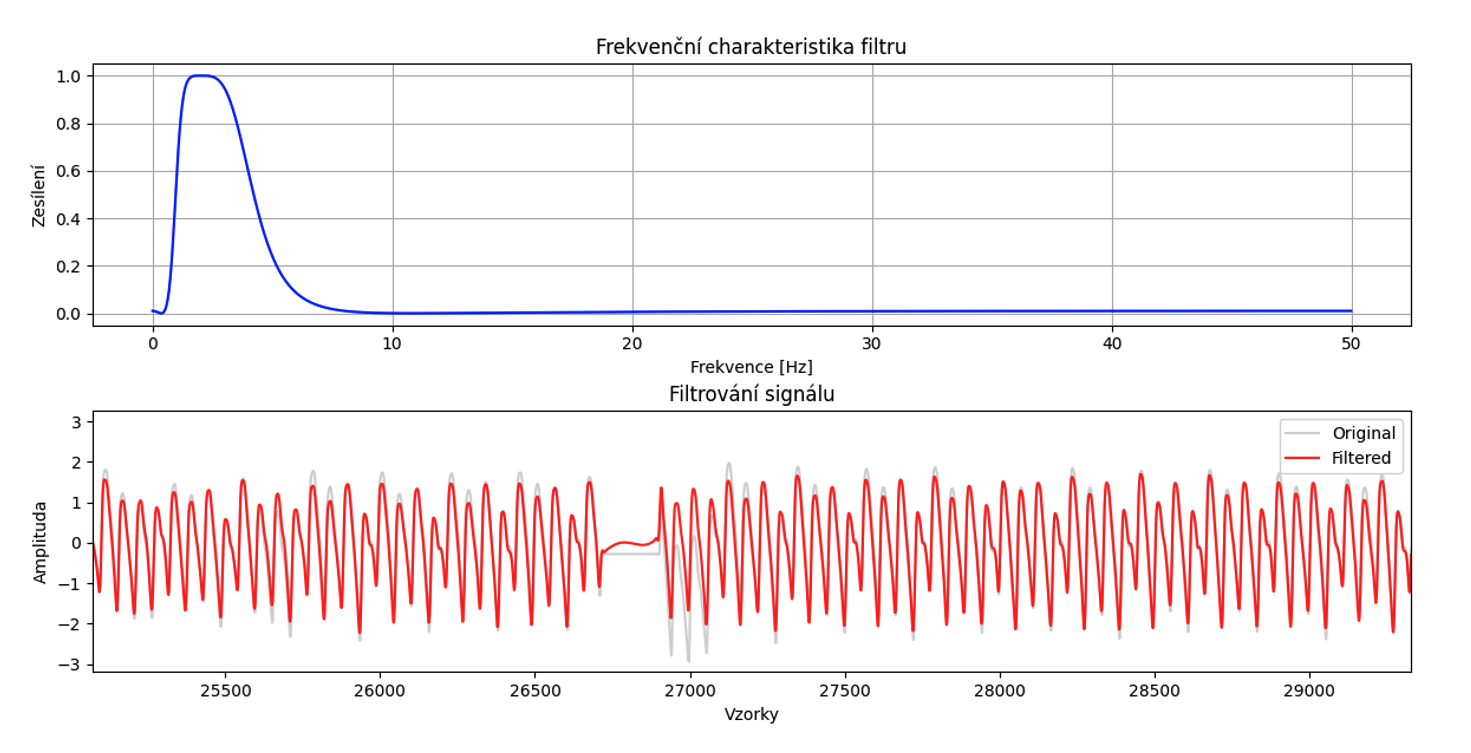
\includegraphics[width=0.8\textwidth]{./obrazky/ElgendiBandpass.png}
	\caption[Filtrace PPG signálu]{Horní graf: příklad amplitudové přenosové charakteristiky pásmové propusti. Dolní graf: znázornění filtrace PPG (šedě původní signál, červeně po filtraci).}
	\label{fig:filter-example}
\end{figure}

\section{Umocnění signálu}
Po filtraci se signál umocňuje na druhou, aby se zdůraznily rozdíly mezi systolickou vlnou a ostatními složkami (například diastolickými zářezy).
Výsledná hodnota $y[n]$ po umocnění je:
\begin{equation}
	y[n] = x[n]^2,
	\label{eq:square}
\end{equation}
kde $x[n]$ je již zfiltrovaný signál. V~důsledku toho bývá systolický vrchol zřetelnější, jak je ilustrováno na obrázku~\ref{fig:squared-signal}.

\begin{figure}[htbp]
	\centering
	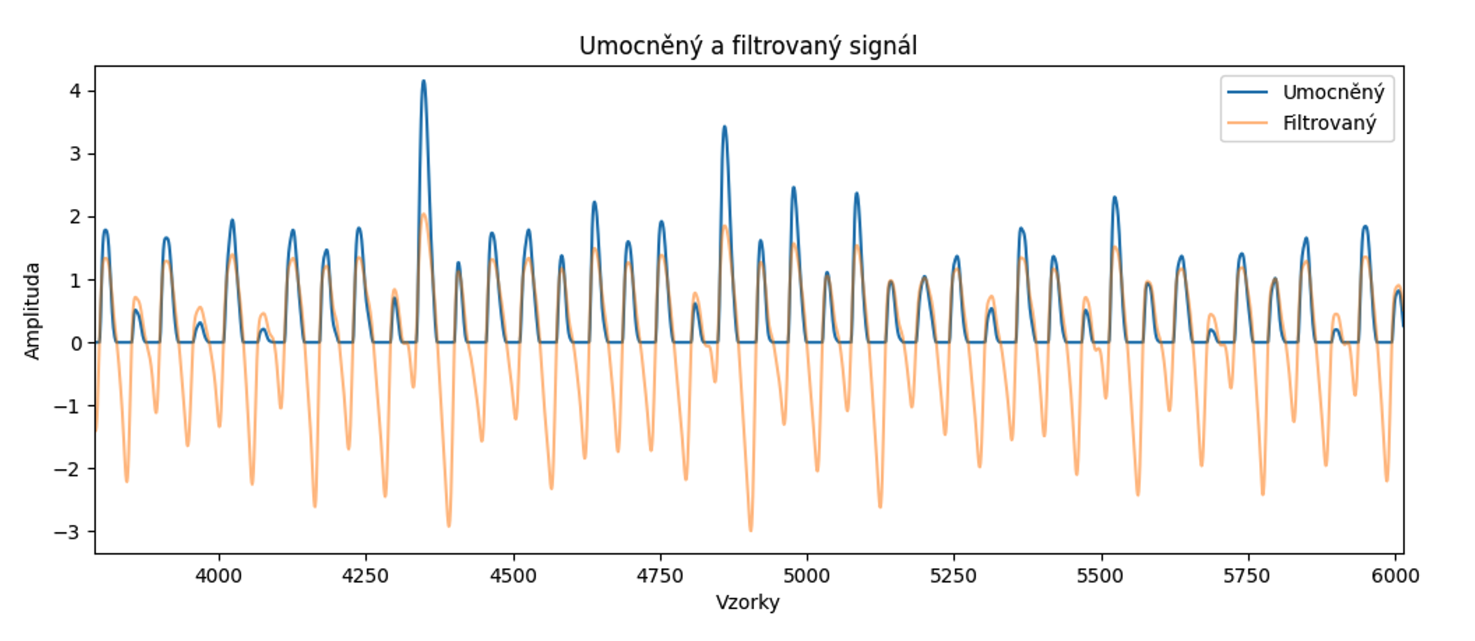
\includegraphics[width=0.8\textwidth]{./obrazky/ElgendiUpravenySignal.png}
	\caption[Umocněný a filtrovaný PPG]{Porovnání filtrovaného PPG a po umocnění.}
	\label{fig:squared-signal}
\end{figure}

% \section{Dvoufázové prahování a nalezení vrcholů}
% Po umocnění je nutné určit, kde přesně hledat potenciální maximum.
% Elgendiho algoritmus často využívá dvě různé délky klouzavého průměru: 
% \begin{itemize}
%  \item Krátké okno, které přibližně odpovídá šířce systolické vlny.
%  \item Delší okno, jež pokrývá přibližně délku celého srdečního cyklu.
% \end{itemize}
% Na základě jejich rozdílu a adaptivních prahů se definují bloky, kde by mohl ležet vrchol. V takto vymezeném úseku se bere maximum jako systolický vrchol. Souhrnně lze postup vyjádřit rovnicí
% \begin{equation}
% 	\text{blok}[n] = \begin{cases}
% 		1 & \text{pokud } \overline{y}_{\text{krátké}}[n] > \overline{y}_{\text{dlouhé}}[n] + \text{offset}, \\
% 		0 & \text{jinak},
% 	\end{cases}
% 	\label{eq:thresh}
% \end{equation}
% kde $\overline{y}_{\text{krátké}}$ a $\overline{y}_{\text{dlouhé}}$ jsou hodnoty klouzavých průměrů ve vzorku $n$ a \emph{offset} je tepově závislá konstanta. Vše je schematicky zobrazeno na obrázku~\ref{fig:block-detection}.

% \begin{figure}[htbp]
% 	\centering
% 	\includegraphics[width=0.78\textwidth]{blocks_detection.jpg}
% 	\caption[Oblasti hledání vrcholů]{Zobrazení umocněného signálu (tmavě modře), filtrovaného signálu (světle modře) a dvou klouzavých průměrů (zelené křivky). Šedé pruhy znázorňují vybrané úseky (bloky), kde hledáme maximum jako systolický vrchol (červené body).}
% 	\label{fig:block-detection}
% \end{figure}

% Aby se předešlo vícenásobné detekci blízko sebe, zavádí se také minimální vzdálenost mezi detekovanými vrcholy. Tato vzdálenost je obvykle nastavena podle reálné fyziologie, např. 200~ms při klidové tepové frekvenci.

% \section{Integrace do NeuroKit2}
% Popsaný postup je implementován v knihovně NeuroKit2 volbou \verb|method="elgendi"| při volání funkce \verb|ppg_process|:
% \begin{verbatim}
% import neurokit2 as nk

% signals, info = nk.ppg_process(
% 	ppg_signal, sampling_rate=fs,
% 	method="elgendi",
% 	method_quality="templatematch"
% )
% \end{verbatim}
% Výstup \verb|signals| typicky obsahuje sloupec s~pozicemi vrcholů a okamžitými hodnotami TF, zatímco \verb|info| nese další kontextové informace, například seznam indexů vrcholů či parametry filtrace.

% \section{Zhodnocení kvality signálu}
% Metoda \verb|templatematch| porovnává tvar každého detekovaného pulzu s~referenční šablonou a vyhodnocuje, do jaké míry odpovídá typické morfologii PPG. Takový přístup zjišťuje, zda je příslušný úsek skutečně “kvalitní” a nemá výrazné artefakty. Výsledkem může být číselné skóre kvality nebo binární označení (kvalitní / nekvalitní).

% \section{Závěr}
% Elgendiho algoritmus, s~částečnými modifikacemi v NeuroKit2, nabízí robustní a do značné míry automatizované řešení detekce systolických vrcholů v PPG. Díky adaptivním prahům a využití dvou klouzavých průměrů dokáže úspěšně potlačit různé formy šumu a spolehlivě najít systolický vrchol. K~praktickému použití navíc poslouží modul \emph{Template-Matching}, který vyhodnotí důvěryhodnost každého detekovaného pulzu.

